\documentclass[12pt]{article}
\usepackage[utf8]{inputenc}
\usepackage{amssymb}
\usepackage{wasysym}
\usepackage[a4paper, margin=2cm]{geometry}
\usepackage[dvipsnames]{xcolor}
\usepackage{graphicx}
\graphicspath{ {./PoC Scoping Exercise/} }
\usepackage{scrextend}


\title{\textbf{Learning Journal}}
\date{Date of last edit: \today}
\author{William Black 42920477}
\setlength{\parindent}{0pt}
\setlength{\parskip}{0.5em}

\usepackage{hyperref}
\hypersetup{
    colorlinks=true,
    linkcolor=blue,
    filecolor=magenta,      
    urlcolor=cyan,
}
 
\urlstyle{same}

\begin{document}

\tableofcontents

\newpage\section{11.08.19 - Scoping Exercise I}

Doing the Scoping Exercise first because the other task is recommended to be tackled in groups.

Time to find out how to use LaTeX.

\subsection{LaTeX}

First learning journal will be in Word since I don’t know how to use LaTeX yet.

Brian said to work in Rich Text and watch it come out perfectly on the right.

\subsubsection{\underline{Rich Text Mode Errors:}}\label{error:er1}
\begin{itemize}
    \item Rich text mode in Overleaf does not come out perfectly on the right at all
    \item Sometimes code appears on the Rich Text version of the left
    \item The rich text options are extremely limited, it seems to just be bold, underline, bullet lists, and nothing else
\end{itemize}
\begin{itemize}
\renewcommand{\labelitemi}{$\nobullet$}
\item \underline{Solution:}
\renewcommand{\labelitemi}{$\bullet$}
    \item Don’t use Rich Text mode
\end{itemize}

Brian linked a \href{https://www.overleaf.com/learn/latex/Creating_a_document_in_LaTeX}{tutorial} for using Source mode.

Tutorial going smoothly.

Replacing parts of the tutorial result to reflect my Scoping Exercise.

Worked out using $\backslash$date\{$\backslash$today\} instead of typing out the date, magic!

\subsubsection{\underline{Bullet List Errors:}}\label{error:er2}
\begin{itemize}
    \item Can’t work out how to make nested bullets.
\end{itemize}
\begin{itemize}
\renewcommand{\labelitemi}{$\nobullet$}
\item \underline{Solution:}
\renewcommand{\labelitemi}{$\bullet$}
    \item \href{https://www.overleaf.com/learn/latex/Lists}{This tutorial} shows how to make nested bullets. Since I can, as a learning exercise, I want to combine bullets, bullets, and numbered lists.
\end{itemize}

I’m numbering the parts of my methodology, including the writing process and the bibliography creation. The pains and pain relievers can be bullets.

\href{https://www.overleaf.com/learn/latex/Lists}{The same tutorial} even shows how to change bullet list styles

\href{http://www.rpi.edu/dept/arc/training/latex/LaTeX_symbols.pdf}{This .pdf} is a list of different symbols I can use. 

\subsubsection{\underline{Package Errors:}}\label{error:er3}
\begin{itemize}
    \item Not working. Some of them work but most of them don’t.
\end{itemize}
\begin{itemize}
\renewcommand{\labelitemi}{$\nobullet$}
\item \underline{Solution:}
\renewcommand{\labelitemi}{$\bullet$}
    \item \usepackage{} With the package the symbol is from was surprisingly easy. I assumed I had to install something but just naming the package seems to work. 
    \item I wonder why they don’t just put something like “$\backslash$usepackage\{allpackages\}” at the beginning, and why not make that automatic?
\end{itemize}
    
Just realised I have to write gains and gain creators too, and I have the perfect bullet symbols for them. 

I kind of feel like some sort of genius hacker using LaTeX but my brain is starting to hurt, I’ve been fiddling around with the source editor for a few hours now.
There’s an option to collapse lists at the line numbers when you’re done writing them. It’s much easier to read. I’ve also realised I can separate the lines with single line breaks and nothing changes in the result, which also makes the code much more readable.

\subsubsection{\underline{Right Alignment Errors:}}\label{error:er4}
\begin{itemize}
    \item Even with \href{https://www.overleaf.com/learn/latex/Text_alignment#Right-justified_text}{a tutorial} I can’t make a package work to allow me to make the date right-aligned and smaller.
\end{itemize}
\begin{itemize}
\renewcommand{\labelitemi}{$\nobullet$}
\item \underline{Solution:}
\renewcommand{\labelitemi}{$\bullet$}
    \item 
\end{itemize}
    
Can’t figure out any solution to that problem so I’ll just leave it as is. I wanted to make the date a little less front-and-centre, but maybe the package isn’t working because it’s in the preamble.

But now it looks like I can change the format of the title, so that’s not the rule. \href{https://www.overleaf.com/learn/latex/Font_sizes,_families,_and_styles}{This tutorial} explains how to change font sizes, but rather than “12pt” etc it’s just larger or smaller than the size set at the beginning of the document.

Came across \href{https://www.overleaf.com/learn/latex/Paragraph_formatting#Reference_guide}{this tutorial} that tells me how to fix the automatic indenting. Looks nicer without it.


\subsubsection{\underline{Document Style Errors:}}\label{error:er5}
\begin{itemize}
    \item The margins look kind of insane, they’re like two inches wide, and for some reason they’re even wider on only the second page. The first and third page look normal though.
\end{itemize}
\begin{itemize}
\renewcommand{\labelitemi}{$\nobullet$}
\item \underline{Solution:}
\renewcommand{\labelitemi}{$\bullet$}
    \item After a lot of messing around with this tutorial to use the geometry package to make the margins more normal, I realised two-sided letter paper was still the document style set from when I was going through the set-up tutorial. I’ve made the paper A4 and one-sided.
\end{itemize}

While I don’t think these specific skills are necessarily going to be so handy in creating the ultimate Proof of Concept submission, learning how to search for things I don’t know how to do and familiarising myself with the logic of the program has been a difficult learning curve that I’m enjoying being on top of.

I’m finding it extremely confusing, how to submit the document. Someone else in class has submitted a .tex file, and now I reread the instructions, it does say specifically to upload either a .tex file or a word file on to cloudstor, not a .pdf. But there’s no button to download a .tex file, just a .pdf.

Okay an hour later I figure out you have to exit the program, and download a .zip of the file that contains the .tex file. 

Submitted the .tex file to Cloudstor, the .pdf to Turnitin.

Fingers crossed that next week’s task will take less than 6 hours now I’m more familiar with the program.

\subsection{Business Analysis: Pains and Gains}
The jobs involved in writing the project come down to methodology: Data collection; Contrastive linguistic comparison; Structural linguistic analysis; Writing the thesis. I wouldn't normally put a bibliography in there but since it's the one that keeps coming up as the example I can sense that this might end up being a relatively easy fallback for most students.

The pains and gains are tough to separate, obviously avoiding pain is a gain in itself.

There's no way for me to know whether any of these pain relievers/gain creators are possible to create programs for but this is apparently only to brainstorm, so we are pretending we live in a semi-magic world where small magics are possible, but not magic that's big enough to just do the entire thesis for me. Harry Potter rules.

\newpage
\section{12.08.19 - Data Carpentry}
Since yesterday’s task was so surprisingly complicated, I might see how I do with Data Carpentry solo and keep the tricky parts to ask my friends tomorrow.

\subsection{\textbf{\href{https://datacarpentry.org/spreadsheets-socialsci/00-intro/index.html}{Introduction}}}
\setlength{\parskip}{0.5em}


\color{Gray}\textbf{{Questions}}
\newline What are basic principles for using spreadsheets for good data organization?

\textbf{{Objectives}}
\newline Understand how to organize data so computers can make the best use of the data

\begin{itemize}
\renewcommand{\labelitemi}{$\nobullet$}
\item \textbf{\underline{Exercise}}
\renewcommand{\labelitemi}{$\bullet$}
    \item How many people have used spreadsheets in their research?
    \item How many people have accidentally done something that made them frustrated or sad?
\end{itemize}\color{black}

I’ve used spreadsheets in research quite simply, just to find average values, or added values. A couple of times I tried to test for a null hypothesis, because I had just done Statistics 102 and I could still remember how to do it, but that was very complicated and I’m not 100\% confident doing it again now.

I don’t know if I’ve had that situation in the context of research… a few times a Windows update has interrupted me during an exam, which is scary, but I’ve just taken photos to prove I had a technical error. Definitely the worst one is when a Windows update restarts my computer and I’ve forgotten to save my Word file. It’s fine if you’ve saved it once, because AutoSave saves it for you, but if you haven’t saved and named it yet AutoSave doesn’t run.

\subsection{\textbf{\href{https://datacarpentry.org/spreadsheets-socialsci/01-format-data/index.html}{Formatting Data in Spreadsheets}}}

\\\color{Gray}\textbf{{Questions}}
\\ What are some common challenges with formatting data in spreadsheets and how can we avoid them?

\textbf{{Objectives}}
\\Recognise and resolve common spreadsheet formatting problems.
\\Describe the importance of metadata.
\\Identify metadata that should be included with a dataset.
\color{black}

\vspace{1em}
\textbf{Data formatting} – always prioritise the computer understanding the data over you understanding it. You may need to format differently for different objectives.

\textbf{Keep track of analyses} – never clean/analyse/mess around with your original data, make a copy in a new tab/file and mess with that. Open the next tab to keep notes on what you did to end up with the new version, because you won’t remember in six months.

\textbf{Structuring data} – variables in columns, observations in rows, split all combined observations to simplest possible. When exporting cleaned data, use text-based format like comma-separated values (CSV)

\newpage
\color{gray}
\begin{itemize}
\renewcommand{\labelitemi}{$\nobullet$}
\item \textbf{\underline{Exercise}}
\item We’re going to take a messy version of the SAFI data and describe how we would clean it up.
\end{itemize}
\begin{enumerate}
    \item Download the messy data.
    \item Open up the data in a spreadsheet program.
    \item Notice that there are two tabs. Two researchers conducted the interviews, one in Mozambique and the other in Tanzania. They both structured their data tables in a different way. Now, you’re the person in charge of this project and you want to be able to start analyzing the data.
    \item With the person next to you, identify what is wrong with this spreadsheet. Discuss the steps you would need to take to clean up the two tabs, and to put them all together in one spreadsheet.
\end{enumerate}
\color{black}

\begin{enumerate}
    \item Downloaded.
    \item Opened.
    \item Noticed tabs.
    \item There are too many things wrong with the data to just clean or fix. Some farmers would need to be re-interviewed or excluded from the sample if there’s no recording of the interview. Problems and solutions where possible listed below.
\end{enumerate}

\textbf{{Mozambique Data:}}
\begin{itemize}
\renewcommand{\labelitemi}{$\nobullet$}
    \item \underline{Dwellings}
\renewcommand{\labelitemi}{$\bullet$}
    \item Some typos – mabati\_sloping instead of mabatisloping, errth instead of earth
    \item Most of the columns do not have spaces, presumably for algorithm reasons. “wall type”, “floor type”, “water use” should have their spaces replaced with underscores if that’s necessary.
    \item Farmer #3 has -99 rooms in his dwelling, which is arguably too few.
    \item Farmer #10 has five rooms in his dwelling including a barn. If the barn doesn’t count as a room, there should be a separate column for barns.
\renewcommand{\labelitemi}{$\nobullet$}
    \item \underline{Livestock}
\renewcommand{\labelitemi}{$\bullet$}
    \item Farmer #10 has no entry. If he has no livestock, it should say he has 0 so he is still included in the sample. Also check whether the missing entry really belongs to Farmer #10, or if it is another farmer whose absence has moved the other farmers up a position in key\_id
    \item The number of livestock owned appears to be automatically generated from how many comma-separated animals are listed. This means that the number represents the number of TYPES of livestock owned, not the number of livestock. If number of livestock is needed, the farmers need to be re-interviewed and columns for each type of livestock should be made to record numbers of each type.
    \item Where “none” was entered, “1” type of livestock was recorded because the program assumed a none was a type of livestock. “none” entries should be replaced with “0”.
    \item Farmer #10 has five rooms in his dwelling including a barn. If the barn doesn’t count as a room, there should be a separate column for barns. 
    \item For Farmers #1 and #5, “poultry” was counted as a type of livestock, where it was not for the other farmers.
    \item It is quite unlikely that Farmers #2, #4, #5, and #9 own cows but don’t look after them. Perhaps someone else has removed that responsibility from them but the researcher should check if that’s true.\renewcommand{\labelitemi}{$\nobullet$}
    \item \underline{Plots}
\renewcommand{\labelitemi}{$\bullet$}
    \item “yes” and “no” are not consistent. Ideally, these values should be replaced with binary “1” = yes and “0” = no, or "yes" and "no".
    \item Farmers #5 and #10 have not had plots recorded. If they have no plots, “0” should be recorded.
    \item Where “none” was entered, “1” type of livestock was recorded because the program assumed a none was a type of livestock. “none” entries should be replaced with “0”.
    \item Farmer #9 has -999 plots on his farm, which is arguably too few.
    \item Farmer #2 only uses water during summer. If this affects the data, columns should be made for the seasons of Mozambique and Tanzania to record water usage in each season. If it does not affect data, then the most accurate answer is “yes”.
\end{itemize}

\textbf{{Tanzania Data:}}
\begin{itemize}
\renewcommand{\labelitemi}{$\nobullet$}
    \item \underline{Dwellings}
\renewcommand{\labelitemi}{$\bullet$}
    \item If wall type, floor type, and look after cows categories should not have spaces in their cells, replace spaces with underscores.
    \item Farmer #8 has 4 rooms including a cowshed. If a cowshed is not a room, there should be another column for cowsheds. underscores if that’s necessary.
\renewcommand{\labelitemi}{$\nobullet$}
    \item \underline{Livestock}
\renewcommand{\labelitemi}{$\bullet$}
    \item Farmer #10’s entry is missing. If he has no livestock then “0”s should be recorded. Also check whether the missing entry really belongs to Farmer #10, or if it is another farmer whose absence has moved the other farmers up a position in key\_id.
    \item Many values are not recorded. If there are no livestock of that category, 0 should be recorded.
    \item Many of the totals do not equal the number of livestock recorded. Farmers need to be re-interviewed for correct numbers.
    \item Farmers #4 and #9 have cows and do not look after cows, which seems unusual. Researcher should check if that’s true.
    \item Farmer #3 had a cow that died in April. The data should stipulate whether these values are for total owned during a particular period or a synchronic analysis. If the cow-owning was during the period, the Cows value should read “1”, and look\_after\_cows should read “yes”. If the number are only to reflect the situation at interview, look\_after\_cows should read “no”.
\end{itemize}

\textbf{Metadata} – The stipulations on your parameters (what counts as a room, is poultry a livestock, etc). This lesson discourages your from putting this information in the file but I can’t think of any reason putting it in a separate tab wouldn’t be a good idea. \color{teal}\small{- (16.08.19) The reason is for future compatibility. When saving in a universal format, tabs aren't saved. If you save in the Excel format, there may be compatibility issues with other programs, or other versions of Excel.}

\color{gray}
\begin{itemize}
\renewcommand{\labelitemi}{$\nobullet$}
\item \textbf{\underline{Exercise}}
    \item Download a clean version of this dataset and open the file with your spreadsheet program. This data has many more variables that were not included in the messy spreadsheet and is formatted according to tidy data principles.
    \item Discuss this data with a partner and make a list of some of the types of metadata that should be recorded about this dataset. It may be helpful to start by asking yourself, “What is not immediately obvious to me about this data? What questions would I need to know the answers to in order to analyze and interpret this data?”
\end{itemize}

\color{black}
\begin{itemize}
\renewcommand{\labelitemi}{$\nobullet$}
    \item The variables need to be defined for a human to read this. Years\_liv might be years at the address, years that the farm has been functioning, years in the village, etc. Months\_lack\_food might be over the past calendar year, the last 12 months, it might be a lack of human food, livestock food, or lack of food produced by the farm
    \vspace{0.5em}
    \newline Affect\_conflicts appears to be a multiple-choice answer, so we need all the options that were available to interviewees.
    \vspace{0.5em}
    \newline Some definitions need to be made like, what counts as a “room” in the dwelling.
\end{itemize}

\newpage\section{14.08.19 – Data Carpentry}

\subsection{\textbf{\href{https://datacarpentry.org/spreadsheets-socialsci/02-common-mistakes/index.html}{Formatting Problems}}}

\underline{Common Spreadsheet Errors}
\begin{itemize}
    \item Using multiple tables
    \begin{itemize}
        \item Confuses the computer, who assumes that Column D will be the same variable for any Row.
    \end{itemize}
    \item Using multiple tabs for like data
    \begin{itemize}
        \item Any information put in separate tabs is not able to interact with earlier tabs, so it wouldn’t be good for things like new measurements of same variables
        \item Under the View menu there’s an option to freeze top row or left column so you can still see them when you’re deep in the spreadsheet
    \end{itemize}
    \item Not filling in zeros
    \begin{itemize}
        \item If you don’t fill in zeros, you don’t know if there are none or if you just haven’t measured the variable yet
    \end{itemize}
    \item Using problematic null values
    \begin{itemize}
        \item Apparently some people put -999 for null values. It’s obvious why that’s not a good idea
    \end{itemize}
    \item Using formatting to convey information
    \begin{itemize}
        \item Don’t add a comment to a cell, the computer can’t read it. If the comment is important to the data, it’s a new variable and needs its own column.
    \end{itemize}
    \item Using formatting to make the data sheet look pretty
    \begin{itemize}
        \item Don’t merge cells, stats software can’t read it
    \end{itemize}
    \item Placing comments or units in cells
    \begin{itemize}
        \item Software can’t read it
    \end{itemize}
    \item Entering more than one piece of information in a cell
    \begin{itemize}
        \item Every aspect of information that’s important is its own variable with its own column. If it’s not important it doesn’t need to be in the cell
    \end{itemize}
    \item Using problematic field names
    \begin{itemize}
        \item No spaces because some software uses spaces as delimiters. No special characters. Numerals are allowed but ideally avoided so they don’t get caught up in your observations. 
    \end{itemize}
    \item Using special characters in data
    \begin{itemize}
        \item To avoid cutting off elements, treat the spreadsheet like a web form that can only contain plain unformatted alphanumerical characters
    \end{itemize}
\end{itemize}


\underline{Problematic Data Produced by my Discipline}

\vspace{1em}
I’m an interdisciplinary student and have three disciplines to choose from, but I’ll go with Media & Communication since this semester is quite focused on that framework in my process.

This isn’t exactly a “bad spreadsheet”, but this is an example of poor design with missing variables that’s bothered me for a few years now – why on earth would movies be ranked or have their success judged based on gross earnings? 

Let’s allow for the argument that we judge merit based on earnings as quantifiable numbers rather than based on unquantifiable “inspiration” or “enjoyment” etc.
 
Here is a spreadsheet of the top-earning films of 2018. 

\vspace{1cm}
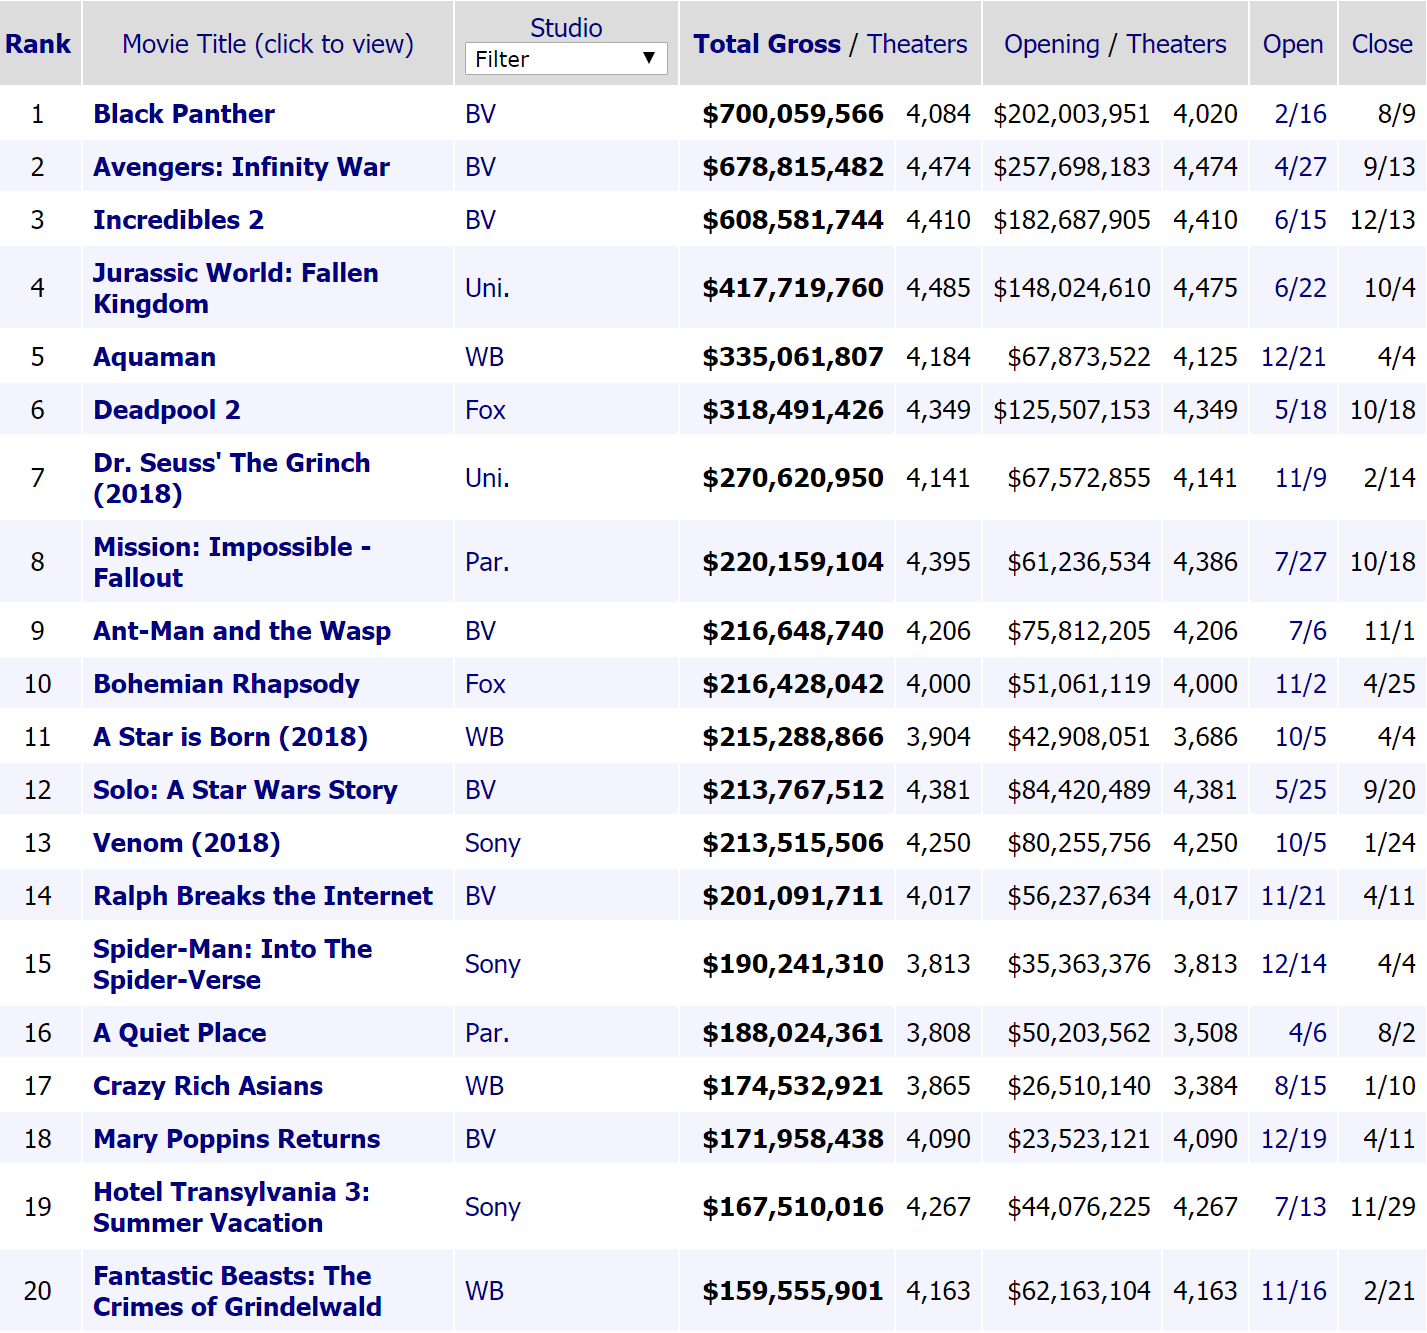
\includegraphics[width=\textwidth]{Topfilms.png}

\vspace{1em}
\newpage
\textbf{Problems:}
\begin{enumerate}
    \item \underline{The films were released at different numbers of cinemas}
    \vspace{0.5em}
    \\For example, A Quiet Place earnt less than Jurassic World, but was available at 3808 cinemas to Jurassic World’s 4485 cinemas.
    \item \underline{The films were released at different cinemas}
    \vspace{0.5em}
    \\Each cinema sets its own ticket price, and has different deals for cheap Tuesdays, discounts, promotional prices with nearby restaurants, etc. The amount grossed does not give any indication of how many audience members saw the film or the success of the film, because there are no numbers on how many cents of each ticket price is taken by the cinema.
    \item \underline{What year they opened and closed}
    \vspace{0.5em}
    \\This is more a problem with the design of the spreadsheet itself than the design of the project, but the dates for opening and closing are ambiguous. I might guess, looking at the numbers, that the dates are formatted mm/dd, but there is no year on either to show how long they were open for. Even though this list is for 2018, there’s no indication whether it is the opening dates or closing dates that occur in 2018. I might guess opening, just based on my background knowledge of the titles in the list, but then it doesn’t necessarily follow that the closing year is 2019, many films may be in cinemas for over a year. Rocky Horror Picture Show is still being played at cinemas since 1975.
    \item \underline{They were open for different lengths of time}
    \vspace{0.5em}
    \\The Grinch did not perform as well as Incredibles 2, but it had literally half the time within which to earn that money. If the data divided the gross by average grossed per day, this would be a very different spreadsheet
    \item \underline{Biggest problem: They have different production budgets}
    \vspace{0.5em}
    \\If we’re happy to commit to financial earnings being our metric for success, amount grossed is not a logical approach. Financial success should tell you what production companies/directors/actors are the safest financial investments for investing distribution companies, portfolios managers, etc., but this does nothing to show what kind of return these titles made on their investments, only how much money was received. 
    \vspace{0.5em}
    \\For a film like Jurassic Park, ranked #4 due to grossing ~\$418 million, the production budget was ~\$170 million, meaning that the amount earnt by the movie was approximately 245\% of its investment. 
    \vspace{0.5em}
    \\A Quiet Place, for comparison, ranked at #16 for grossing \$188 million, but had a meagre production budget of \$17 million, meaning that the film earnt 1,106\% of its investment.
    \vspace{0.5em}
    \\For Fantastic Beasts: The Crimes of Grindelwald, the production was ~\$200 million, meaning that the film actually LOST \$40 million, and yet is ranked #20 on the most successful films of 2018. 
\end{enumerate}

\newpage\section{16.08.19 - Transferring the Learning Journal to Overleaf}

\subsection{LaTeX}
\subsubsection{\underline{Paragraph Spacing Errors:}}\label{error:er6}
\begin{addmargin}[1cm]{0cm}
Struggling to work out how to start a new paragraph rather than new line. 

\underline{Solution:}

New line can be made with just two backslashes without using $\backslash$newline.

New paragraph can be made with $\backslash$par, but isn't a proper paragraph break.

Two enter-breaks can also be used for a paragraph break.

I found an option to $\backslash$parskip\{1em\}. It's a toggle that can be used in the preamble and set through the document.

\textcolor{teal}{- (19.08.19) I saw someone on Slack suggest using $\backslash$vspace\{1em\} for one-off instances of stretching, which is exactly what I was looking for.}


\end{addmargin}

What's an em? \color{teal}{\small{- (19.08.19) An "em" is the space an M takes in the current font. That's quite handy because it's a measurement that changes with the font size.}}

\color{black}
My word document had a lot of hyperlinks, 
\href{https://www.overleaf.com/learn/latex/Hyperlinks}{here} is a tutorial on making hyperlinks. Now I can insert all the hyperlinks I had in the original document

\subsubsection{\underline{Special Characters Errors:}}\label{error:er7}
\begin{addmargin}[1cm]{0cm}
I'm having a problem with special characters in Overleaf such as \% and \$ and $\backslash$. They have functions in Overleaf so I can't use them as text characters without them performing their functions.

\underline{Solution:}

I worked out you can use a backslash before most of the special characters to stop them from getting formatted in the main document (thanks, Reddit addiction), but that doesn't work on backslashes. I also can't think of a good way to google that, "how to use backslashes in Overleaf" is only getting me how to use them as a function, of course.
\\\textcolor{teal}{- (19.08.19) Couldn't stay long enough after class to get my questions answered, but found an answer on a forum to insert the $symbol$ of a backslash as \texttt{"\$$\backslash$backslash\$"}.}
\end{addmargin}

\section{19.08.19 - Still transferring the Learning Journal to Overleaf}
\subsection{LaTeX}

\texttt{$\backslash$texttt} makes fonts monospace, I'll keep that going from now on.

I'm starting to get the hang of how to run Overleaf now. You really just google everything you want to do and there's always a tutorial for it somewhere. 

\subsubsection{\underline{Image Insertion Errors:}}\label{error:er8}
\begin{addmargin}[1cm]{0cm}
I'm a bit confused about how to get an image in - I used one for explaining the bad data from my discipline. In Word I just clipped it with the clipping tool and ctrl+Ved to Word. The tutorial seems to have 5 different ways that I understand equally poorly.

\underline{Solution:}

I had to add the package to the preamble. The directory is the directory on Overleaf, not my directory.

You can set the width of the image to equal the text width with 
\\$\backslash$includegraphics[width=$\backslash$textwidth]\{imagefilename\}
\end{addmargin}

\vspace{0.5em}
Wow I didn't realise I had a directory, actually I've put this learning journal in a folder called "Scoping Exercise".

Frankly, I'd like to keep these together so I can easily find codes I used elsewhere. I'll just rename the folder to be all-purpose. "William-Black-Exercises" to avoid spaces.

I also had a look at indenting entire paragraphs before, I wonder if I just forgot a package in the preamble like for the graphics.

Yes I did.

\subsubsection{\underline{Margins Errors:}}\label{error:er9}
\begin{addmargin}[1cm]{0cm}
I want to indent the whole paragraph, not just the first line, because it's quite difficult to read different section that lie in the same space like this.

\underline{Solution:}

I had to add the scrextend package to the preamble. Now I can use $\backslash$begin\{addmargin\}[1cm]\{0cm\} to make left margin 1cm and right margin 0cm, and $\backslash$end\{addmargin\} to indent whole paragraphs.

\end{addmargin}

This is getting a lot easier. I've only spent 2:30hrs on the journal today and I transferred the entire thing including this entry I'm making now.

To be honest, I'm really unaware of any situation where this would be faster or easier than a regular word processor but I'm trusting I'll eventually find one!

\newpage\section{19.08.19 - Data Carpentry}

\subsection{\href{https://datacarpentry.org/spreadsheets-socialsci/03-dates-as-data/index.html}{\textbf{Dates as Data}}}

\color{gray}
\underline{Questions}

- What are good approaches for handling dates in spreadsheets?

\underline{Objectives}

- Recognise problematic or suspicious date formats.
\newline - Use formulas to separate dates into their component values (e.g. Month, Day, Year)
\color{black}

\textbf{Date formats in spreadsheets} - It is $not$ best practice to store dates in one column, ideally you have a day, month, and year column.

\textbf{Dates stored as integers} - Excel stores dates as days from 31 Dec 1899, which can be useful if you need to average durations or study the dates as integers.

\textbf{Regional date formatting} - While there is an option to make date format suit your region, you'll forget to set it or US researchers will forget to adjust it or will try to adjust it when you already did.

\color{gray}
\underline{Exercise:}
\begin{enumerate}
    \item Download and open the dates.xlsx file. This file contains a subset of the data from the SAFI interviews, including the dates on which the interviews were conducted.
    \newline Choose the tab of the spreadsheet that corresponds to the way you format dates in your location (either day first DD\_MM\_YEAR, or month first MM\_DD\_YEAR).
    \item Extract the components of the date to new columns. For this we can use the built in Excel functions:
    \newline =MONTH(), =DAY(), =YEAR()
    \newline Apply each of these formulas to its entire column. Make sure the new column is formatted as a number and not as a date.
    \newline We now have each component of our date isolated in it’s own column. This will allow us to group our data with respect to month, year, or day of month for our analyses and will also prevent problems when passing data between different versions of spreadsheet software (as for example when sharing data with collaborators in different countries).
    \item Using the same spreadsheet, add another data point in the interview\_date column by typing either 11/17 (if your location uses MM/DD formatting) or 17/11 (if your location uses DD/MM formatting). The Day, Month, and Year columns should populate for this new data point. What year is shown in the Year column?
\end{enumerate}
\color{black}
\begin{enumerate}
    \item No problem.
    \item Took me a sec on google to remember how to do this. I'm rusty.
    \item 2019. If you don't put a year, it assumes you want the current one. This means if I am working with data from another unknown year I will need the 3-column system to have a null value for the year.
\end{enumerate}

\textbf{Historical data} - dates from before 31 Dec 1899 are not parsed by Excel. 

\newpage
\subsection{\href{https://datacarpentry.org/spreadsheets-socialsci/04-quality-assurance/index.html}{\textbf{Quality Assurance}}}

\color{gray}
\underline{Question:}

How can we carry out basic quality assurance in spreadsheets?

\underline{Objective:}

Apply quality assurance techniques to limit incorrect data entry.
\color{black}

\textbf{Validating data on input} - Data is restricted to numeric range or controlled vocabulary.

\textbf{Restricting data to a numeric range} - Select the whole column. Data $\rightarrow$ Data Tools $\rightarrow$ Data Validation. You can set it to only allow sensible numbers

\color{gray}\begin{addmargin}[1cm]{0cm}
\underline{Exercise:}

Apply a new data validation rule to one of the other numeric columns in this data table. Discuss with the person sitting next to you what a reasonable rule would be for the column you’ve selected. Be sure to create an informative input message.


\color{black}
I'll assume the years\_farm variable is how many years the interviewee has personally been running their farm. Acceptable answers would be 1-100, as less than a full year would be too short for the research aims, and over 100 would be too old to be running a farm, or a confused interviewer who thinks the question is regarding the farm's existence. I'd only take whole integers, because interviewees may struggle to remember the date they took command of their farm, and then data would vary in specificity.

I made my input message title "Whole years interviewee has run farm (1-100)" which displays when hovering over the cell.
\end{addmargin}

\color{black}
\textbf{Restricting data to entries from a list} - Select variable column $\rightarrow$ Data $\rightarrow$ Data Tools $\rightarrow$ Data Validation again. Allow: List will give you a Source box, where you can list the possible answers separated by commas.

\color{gray}\begin{addmargin}[1cm]{0cm}
\underline{Exercise:}

Apply a new data validation rule to one of the other categorical columns in this data table. Discuss with the person sitting next to you what a reasonable rule would be for the column you’ve selected. Be sure to create an informative input message.

\color{black}
The floor\_type variable has limited possible answers, so I could list "cement, earth". Personally, I don't know enough about floors or rooves or walls to know what options are possible. The input message should list the possibilities.
\end{addmargin}

\color{black}
\vspace{1em}
\section{20.08.19 - Data Carpentry}

\subsection{\href{https://datacarpentry.org/spreadsheets-socialsci/05-exporting-data/index.html}{\textbf{Exporting Data}}}

\color{gray}
\underline{Question:}

How can we export data from spreadsheets in a way that is useful for downstream applications?

\underline{Objective:}

Export data from a spreadsheet to a CSV file.

\color{black}

\textbf{Storing data} - Do not save as the default formats .xls or .xlsx, due to compatibility issues. R packages can often read them but may have issues with newer versions. Even Excel's own rules can change between versions. Save as TSV (Tab-Separated Values) or CSV, so you can even open it in Notepad, but it still works perfectly in Excel. Can't save multiple tabs. Save as $\rightarrow$ .csv. (If the data has commas, remove them or enclose field with double quotes.)

\newpage\section{20.08.19 - Scoping Exercise II}

\subsection{LaTeX}
\vspace{1em}
I'll start the document by copying the code from Scoping Exercise I, so I have all the same formatting, date, author, etc.

\subsubsection{\underline{Automatic Dating Errors:}}\label{error:er10}
\begin{itemize}
    \item Just realised the $\backslash$date\{$\backslash$today\} trick is going to be the wrong date once the date changes.
\end{itemize}
\begin{itemize}
\renewcommand{\labelitemi}{$\nobullet$}
\item \underline{Solution:}
\renewcommand{\labelitemi}{$\bullet$}
    \item When dating work on a continuing document, the date should be written out unless the date is something that will change, such as date last edited.
\end{itemize}

Whoops! I'll keep it at the top of this Learning Journal because then you can see the date of last edit.

\section{23.08.19 - Scoping Exercise II}
\subsection{Understanding Scoping Exercise II}
Feedback on Scoping Exercise I: "It seems like your ideas fall into two broad categories, firstly the collection, transcription, translation and analysis of Disney song lyrics and, secondly, writing and referencing your actual thesis. Either of these would be really interesting and useful to pursue."

I agree that the collection, transcription, translation and (comparative) analysis of Disney song lyrics is essentially the mission of the research, but can a computer do that?
 
After staring at these instructions for a couple of hours, here are all the things I don't understand:
\begin{itemize}
    \item Is Scoping Exercise II supposed to find one specific problem to solve or is "collection, transcription, translation, and comparative analysis" a problem I can solve if I can define the boundaries well enough?
    \item The general feedback from the marker: "Part of the scoping process, which was not so well done in the assignment, is the part where students narrow their focus in to one individual idea or group of ideas, ie the pain / gain which you are going to work on this semester as your Proof of Concept / Technology Deployment." 
    
    We were not told to do this in the instructions for Scoping Exercise I, and we \textit{are} told to do this for Scoping Exercise II. If this was the aim of Scoping Exercise I, then what is the required elaboration in Scoping Exercise II?
    \item More feedback: "A number of you jumped straight into finding solutions for your pains / gains, without fully identifying the boundaries of what you are attempting to do. Defining what is both inside and, just as importantly, outside the scope of your project is a key step that will save you both time and frustration."
    
    What is a pain reliever or a gain creator if not a solution to a pain or gain? Identifying the boundaries of what I'm attempting to do is absolutely something that can't be skipped, but the exercise was said to be to "brainstorm" what barriers occur in my research and what it would look like to remove them.
    \item How wishful am I supposed to be with a tool that assists me with research? Since I've no idea what a computer can or can't help with, I don't know how to create a realistic tool, and it seems like there should be some boundaries on how wishful my tool should be.
    
    I suggested that my tool could collect, transcribe, translate and analyse the comparison of the translations, which Brian said looked "great". I assume a computer can't do that though, so what's to stop me aiming for a tool that automatically writes the thesis for me?
    
    \item I cannot understand the Rubric for this task at all. It seems like the Rubric is designed to cover the entire process up to submission at the end of semester, but there is no indication which parts cover which individual tasks.
    
    \item I have found this in the Week 3 Summary: "Scoping Exercise Deadline: Firstly, the initial scoping exercise is due on Sunday 18 August at 11.59pm. This task will be assessed and is the first milestone of your Proof of Concept or Technology Deployment (PoC/TD). The scoping exercise should be submitted via Turnitin. The rubric for the scoping exercise is the first *three* lines of this document [the rubric] and further information on how to approach this assignment and what is required can be found in the 'Proof of Concept Scoping 101' section of the week 2 lecture slides."
    
    As far as I was aware, this task was due on Friday, and I had already submitted it. The explanation of what part of the rubric is used to mark us has to be given before we start the task, not after we submit it. Even giving this explanation on Friday and giving an extension until Sunday is not adequate - I had no notice and I was working 6:00-19:00 that weekend!
    
    What part of the rubric is for this task?
    
    \item This task is not being graded, so does it have a rubric? If not, should I just interpret the instructions in a way that makes sense?
    
    \item Found this message on Slack: 
    \begin{itemize}
    \renewcommand{\labelitemii}{$\nobullet$}
        \item \texttt{Brian 4:39 PM}
        \item Important trap. At the end of the unit, during the final submission for the proof of concept, for the HD "Demonstration of Capability" I wrote: "Proof of Concept achieves goals articulated in the scoping document using tools and techniques tested in elaboration. PoC runs without errors and credibly demonstrates a route for implementation in planned research. PoC matches the product described in the OSP exactly."
        \\So while this is not being graded, it's important to take it seriously
    \end{itemize}
    So the tools and techniques I... "test" in Scoping Exercise II must be used to achieve a goal I specified in Scoping Exercise I? That's just a guess, because:
    \begin{itemize}
        \item Nothing has been labeled as "scoping document" or "elaboration". What do these terms mean?
        \item There is nothing in the instructions for Scoping Exercise II that instructs me to test tools or techniques, only to "decompose" a problem, "recognise patterns" in the data, and to "design an algorithm". If I am supposed to test tools and techniques, that needs to be in the instructions.
        \item We have no idea what the OSP is yet. All we have from the unit guide is "You will write an 'Original Software Publication' (OSP) article appropriate for a software journal detailing your analytic pipeline using the TeX SoftwareX article template provided."
% Original Software Publication is a type of journal article.        
        ... Write an article? Which is it, an article or a software publication? 
        - What's an analytic pipeline? 
    \end{itemize}
    \item The \href{https://unitguides.mq.edu.au/unit_offerings/95891/unit_guide#assessment_task_257486}{unit guide} for this course only specifies four gradeable tasks: three in Weeks 12 and 13, and one that is marked weekly (the learning journal). I'm pretty sure the university does not allow changes to this without having a new unit guide approved, and we are not allowed to be graded on other assessments outside those parameters.
    \item The instructions for Scoping Exercise II are in three steps:
    \begin{enumerate}
        \item \textbf{Decomposition:} First (and most important), decompose the activities that involve ‘pains’, opportunities for ‘gains’, and any solutions you proposed into small parts and/or discrete steps.
        \begin{itemize}
            \item The painful \textit{activities} and gainful \textit{opportunities} are broken down into small steps? How do you do that? 
            \begin{itemize}
                \item Pain: Translating a Japanese lyric set 
                \\Step 1: Get the lyrics from online somewhere 
                \\Step 2: Translate the first line
                \\Step 3: If unknown kanji appears, look it up on jisho.org
                \\Step 4: If line does not appear to make sense, check for other meanings on weblio.jp
                \\Step 5: If line still does not appear to make sense, google the phrase in quotes to see other contexts in which it's used if it's a common phrase, or sometimes if it's an uncommon phrase a native Japanese person will be asking what the phrase means online.
                \\Step 6: Translate next line
                \\Repeat Steps 3-6.
                \vspace{0.5em}
                \item Gain: It would be great if lyrics were already checked for accuracy
                \\Step 1: That would be great.
                \vspace{0.5em}
                \item Gain: It would be great if a program could automatically fill an Excel sheet formatted to equal bar length so I could assign fidelity values to line pairs easily.
                \\Step 1: The program would retrieve the lyrics
                \\Step 2: It would format the lyrics to equal bar length
                \\Step 3: It would fill an Excel sheet with Spanish, English, and Japanese variable columns for each line of song in rows.
                \\Step 4: That would be great.
            \end{itemize}
            \item Also any \textit{solutions} I proposed in Scoping Exercise I are broken down in to small steps
            \begin{itemize}
                \item Firstly, the marker gave us feedback that we were NOT supposed to come up with solutions in Scoping Exercise I
                \item How do you break down a solution that doesn't exist/doesn't exist yet into smaller steps?
                \vspace{0.5em}
                \item Gain creator: A program that could listen to music and autogenerate the lyrics in any language.
                \\Step 1: Learn how to make program
                \\Step 2: Use newfound skill to make the program
                \\Step 3: Run the program
                \vspace{0.5em}
                \item Obviously breaking this down doesn't make sense because I don't know what steps are involved apart from "find out what steps are involved". And I don't know if this is possible with current technology, so I also don't want to be penalised later when I can't fulfil my stated goal.
                \end{itemize}
        \end{itemize}
        \item \textbf{Pattern Recognition:} Next (if possible), identify patterns in the problems you are trying to solve or the solutions you are proposing.
        \begin{itemize}
            \item If possible? So this part is not a requirement? 
            \item Earlier in the same instructions, Pattern Recognition was about recognising patterns in data, not in problems or solutions. Is it data, or problems and solutions?
            \item The real pattern for all of them is that I don't know how to solve the problems, if they can be solved, or what steps one might take to solve them.
        \end{itemize}
        \item \textbf{Algorithm Design:} Finally, revise the solutions you developed during Business Analysis to produce a step-by-step guide describing what you want to accomplish.
        \begin{itemize}
            \item First of all, the marker gave us feedback on Slack that we were NOT supposed to come up with solutions in Scoping Exercise I.
            \item What is Business Analysis? - I asked Brian on Slack and he confirmed Business Analysis is another name for Scoping Exercise I.
            \item How can a step-by-step guide that "describes a goal" be produced? I guess maybe it means a step-by-step guide to \textit{achieving} the goal, but that doesn't make sense either because how can I magically know how to achieve a goal I'm not even sure is possible to achieve? If I knew what the solution to the pain point was, obviously it wouldn't be a pain point because I would just carry out that solution. 
        \end{itemize}
    \end{enumerate}
    \item Although it doesn't say in the instructions (it should REALLY say this in the instructions!!), more information from Slack suggests we are supposed to focus on ONE specific, useful, achievable proof of concept/tech demonstration.
    \begin{itemize}
        \item How can a proof or a demonstration be specific, useful, and achievable? I think I STILL don't know what a proof of concept or a tech demonstration is.
        \item Does this mean the PoC and the TD are the same thing? Because they are two separate assignments in this course
        \item Brian elaborates, "We're taking all of the possible problems you could solve and finding one that is worthy of solving in the time available." How am I to know what problem is worthy? How am I to know what problem can be solved within 10 weeks? How am I to know what problem can be solved? Am I supposed to guess? If I guess wrong, my marks for the assessment suffer because I didn't use the techniques and tools that I was supposed to "test" in this exercise. - Whatever "test" might mean in this context.
    \end{itemize}
    \item Am I the one that's insane here? I know from 4 years of university study that usually when I'm confused, everyone else is just as confused as me but less likely to articulate it and be specific about it than I am. But still. This is a LOT of people who would be just guessing what to do and are satisfied with whatever result comes. Surely someone else is concerned about this??
\end{itemize}

\section{26.08.19 - Scoping Exercise II}
\subsection{Computational Analysis: Decomposition, Patterns, Algorithm Design}
Now I've had my questions cleared up by Shawn and Brian I can start the task. 

\textbf{Decomposition}

I should break down the pains/gains I listed in Scoping Exercise I into a step-by-step process of what I currently have to do for each pain manually, into as many steps as would be required for a researcher from a different discipline to be able to follow. 

Hard to know exactly how far to decompose this, because for something like data acquisition, for mine I would certainly need to a bunch of things to decide how to SELECT what data to acquire. 

I'll try to cover everything I can think of, it won't matter if it's overkill because Pattern Recognition stage will work out what's useful.

\newpage
\subsubsection{\underline{Displaying Japanese Characters Errors:}}\label{error:er11}
\begin{itemize}
    \item None of the Japanese characters are displaying when I compile the code.
    \item A lot of the suggestions I'm finding online for typing in Japanese are suggesting packages that don't work, perhaps because they are designed for things called "XeTeX" or "pTeX" or "LuaLaTeX", which I'm guessing might be a different format to LaTeX
\end{itemize}
\begin{itemize}
\renewcommand{\labelitemi}{$\nobullet$}
\item \underline{Solution:}
\renewcommand{\labelitemi}{$\bullet$}
    \item I finally found a \href{https://tex.stackexchange.com/questions/68333/how-to-put-japanese-kanji-characters-into-an-english-document}{forum support question} that specifically asks how to insert Japanese characters into English documents.
    \item Although the answer at this link is incorrectly formatted, the package CJKutf8 does work, if you begin and end \texttt{\{CJK\}\{UTF8\}} and \texttt{\{Japanese\}} around the begin and end lines of \texttt{\{document\}}.
\end{itemize}

\textbf{Pattern Recognition}

Although I expected to need to pick one or two favourites out of perhaps 6 possible robots, the decomposition process has resulted in two neat categories: Getting canon lyrics automatically populated to a spreadsheet ready for me to analyse; and helping me write and reference my research the way I want.

I remember Shawn said the first process may not be as difficult as I think, but it's awfully niche-use. If I could really make a framework that would help me stay on my writing, I could use that for every thesis I ever write, which would be amazing. I suppose PoCs for citations are kind of the "fallback" PoC project for this class, but I'm really tempted by this one because it would also \textit{organise} me which is my main barrier of ADHD to overcome. Doing it by hand as I do now is extremely effective but it does take a lot of extra time.

\textbf{Algorithm Design}

I didn't realise until typing this out how great a writing frame would be, I really want that to exist already so I can use it for my 6000 word essay this semester. 

I wonder how difficult it would be to make something visual like that? I'm an ex-graphic designer, I could make it look cute to use and everything. 

I also wonder how possible it would be to make something that interacts with... Word, say. I suppose you ought to avoid making something that is at the mercy of Microsoft's current version of Word, but I'm not about to be capable of making my own word processor either.

\newpage\section{Library of Errors}
\begin{enumerate}
    \item Rich Text Mode \ref{error:er1}
    \item Bullet List \ref{error:er2}
    \item Using Packages \ref{error:er3}
    \item Right Alignment \ref{error:er4}
    \item Document Style \ref{error:er5}
    \item Paragraph Spacing \ref{error:er6}
    \item Special Characters \ref{error:er7}
    \item Image Insertion \ref{error:er8}
    \item Margins \ref{error:er9}
    \item Automatic Dating \ref{error:er10}
    \item Displaying Japanese Characters \ref{error:er11}
\end{enumerate}

\end{document}

% commit details: what was added, deleted, changed, AND how it went